\begin{frame}
  \frametitle{Don't cut down the trees}
\begin{itemize}
\pause
\item Tree: a connected undirected graph with no cycles
\pause
\begin{example}
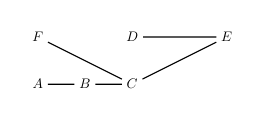
\begin{tikzpicture}[scale=0.6, every node/.style={scale=0.5}]
\node (A) at (1, 2) {$A$};
\node (B) at (2, 2) {$B$};
\node (C) at (3, 2) {$C$};
\node (D) at (3, 3) {$D$};
\node (E) at (5, 3) {$E$};
\node (F) at (1, 3) {$F$};

\draw (A) to (B);
\draw (B) to (C);
\draw (C) to (F);
\draw (E) to (C);
\draw (D) to (E);
\end{tikzpicture}
\end{example}

\pause
\item Forest: one or more trees (my favorite definition in th whole book)
\pause
\begin{example}
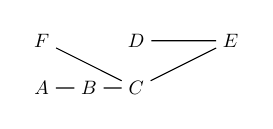
\begin{tikzpicture}[scale=0.6, every node/.style={scale=0.7}]
\node (A) at (1, 2) {$A$};
\node (B) at (2, 2) {$B$};
\node (C) at (3, 2) {$C$};
\node (D) at (3, 3) {$D$};
\node (E) at (5, 3) {$E$};
\node (F) at (1, 3) {$F$};

\draw (A) to (B);
\draw (B) to (C);
\draw (C) to (F);
\draw (E) to (C);
\draw (D) to (E);
\end{tikzpicture}
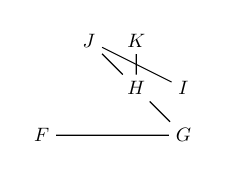
\begin{tikzpicture}[scale=0.6, every node/.style={scale=0.7}]
\node (A) at (1, 2) {$F$};
\node (B) at (4, 2) {$G$};
\node (C) at (3, 3) {$H$};
\node (D) at (4, 3) {$I$};
\node (E) at (2, 4) {$J$};
\node (F) at (3, 4) {$K$};

\draw (A) to (B);
\draw (B) to (C);
\draw (C) to (F);
\draw (E) to (C);
\draw (D) to (E);
\end{tikzpicture}
\end{example}

\pause
\item Rooted tree: same, but one node is `special'
\pause
\begin{example}
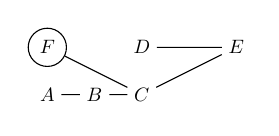
\begin{tikzpicture}[scale=0.6, every node/.style={scale=0.7}]
\node (A) at (1, 2) {$A$};
\node (B) at (2, 2) {$B$};
\node (C) at (3, 2) {$C$};
\node (D) at (3, 3) {$D$};
\node (E) at (5, 3) {$E$};
\node (F) at (1, 3) [circle,draw=black] {$F$};

\draw (A) to (B);
\draw (B) to (C);
\draw (C) to (F);
\draw (E) to (C);
\draw (D) to (E);
\end{tikzpicture}
\end{example}



\end{itemize}
\end{frame}


\begin{frame}
\frametitle{Our favorite kind of trees}
\begin{itemize}
\pause
\item $m$-ary tree (as in binary tree): each vertex has at most $m$ children
\pause
\begin{example}
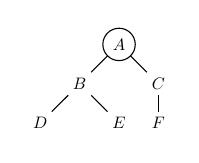
\begin{tikzpicture}[scale=0.5, every node/.style={scale=0.6}]
\node (A) at (3, 0) [circle,draw=black] {$A$};
\node (B) at (2, -1) {$B$};
\node (C) at (4, -1) {$C$};
\node (D) at (1, -2) {$D$};
\node (E) at (3, -2) {$E$};
\node (F) at (4, -2) {$F$};

\draw (A) to (B);
\draw (B) to (D);
\draw (B) to (E);
\draw (A) to (C);
\draw (C) to (F);
\end{tikzpicture}
\end{example}

\pause
\item full binary tree: each vertex has 0 or $m$ children
\pause
\begin{example}
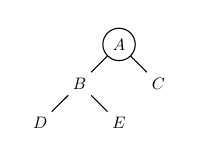
\begin{tikzpicture}[scale=0.5, every node/.style={scale=0.6}]
\node (A) at (3, 0) [circle,draw=black] {$A$};
\node (B) at (2, -1) {$B$};
\node (C) at (4, -1) {$C$};
\node (D) at (1, -2) {$D$};
\node (E) at (3, -2) {$E$};

\draw (A) to (B);
\draw (B) to (D);
\draw (B) to (E);
\draw (A) to (C);
\end{tikzpicture}
\end{example}

\pause
\item Perfect binary tree: every leaf is at the same level
\pause
\begin{example}
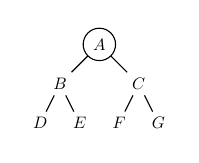
\begin{tikzpicture}[scale=0.5, every node/.style={scale=0.6}]
\node (A) at (3, 0) [circle,draw=black] {$A$};
\node (B) at (2, -1) {$B$};
\node (C) at (4, -1) {$C$};
\node (D) at (1.5, -2) {$D$};
\node (E) at (2.5, -2) {$E$};
\node (F) at (3.5, -2) {$F$};
\node (G) at (4.5, -2) {$G$};

\draw (A) to (B);
\draw (B) to (D);
\draw (B) to (E);
\draw (A) to (C);
\draw (C) to (F);
\draw (C) to (G);
\end{tikzpicture}
\end{example}
\end{itemize}
\end{frame}

\begin{frame}
  \frametitle{Dendrology}
  \begin{itemize}

    \pause
  \item Leaf node:
    \pause a node with no children

    \pause
  \item Internal node:
    \pause a node with children

    \pause
  \item Subtree:
    \pause subgraph that is also a tree

    \pause
  \item Height:
    \pause the longest path from the root to a leaf
  \end{itemize}
\end{frame}

\begin{frame}
\frametitle{Cool things trees can do}
\begin{itemize}
\pause
\item Binary search

\only<2>{
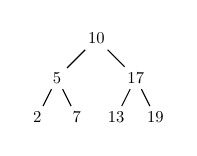
\begin{tikzpicture}[scale=0.5, every node/.style={scale=0.6}]
\node (A) at (3, 0) {10};
\node (B) at (2, -1) {5};
\node (C) at (4, -1) {17};
\node (D) at (1.5, -2) {2};
\node (E) at (2.5, -2) {7};
\node (F) at (3.5, -2) {13};
\node (G) at (4.5, -2) {19};

\draw (A) to (B);
\draw (B) to (D);
\draw (B) to (E);
\draw (A) to (C);
\draw (C) to (F);
\draw (C) to (G);
\end{tikzpicture}
}

\only<3>{
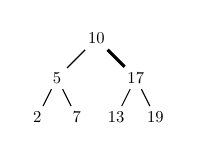
\begin{tikzpicture}[scale=0.5, every node/.style={scale=0.6}]
\node (A) at (3, 0) {10};
\node (B) at (2, -1) {5};
\node (C) at (4, -1) {17};
\node (D) at (1.5, -2) {2};
\node (E) at (2.5, -2) {7};
\node (F) at (3.5, -2) {13};
\node (G) at (4.5, -2) {19};

\draw (A) to (B);
\draw (B) to (D);
\draw (B) to (E);
\draw [very thick] (A) to (C);
\draw (C) to (F);
\draw (C) to (G);
\end{tikzpicture}
}

\only<4->{
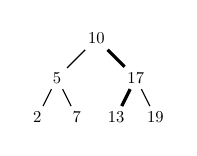
\begin{tikzpicture}[scale=0.5, every node/.style={scale=0.6}]
\node (A) at (3, 0) {10};
\node (B) at (2, -1) {5};
\node (C) at (4, -1) {17};
\node (D) at (1.5, -2) {2};
\node (E) at (2.5, -2) {7};
\node (F) at (3.5, -2) {13};
\node (G) at (4.5, -2) {19};

\draw (A) to (B);
\draw (B) to (D);
\draw (B) to (E);
\draw [very thick] (A) to (C);
\draw [very thick] (C) to (F);
\draw (C) to (G);
\end{tikzpicture}
}

\item<5-> 2 comparisons instead of 5 from linear search

\item<6-> Huffman Coding

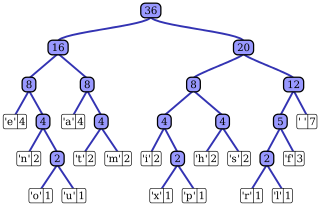
\includegraphics[width=3in]{Huffman_tree.png}
\end{itemize}
\end{frame}

%%% Local Variables:
%%% mode: latex
%%% TeX-master: "graphs"
%%% End:
